\documentclass[Preamble]{subfiles}
\usepackage[english]{babel}
\begin{document}

\chapter{Prototype: School DNS}
A school want to use a DNS server to filter certain internet sites from students and also have the opportunity to get a faster response from the name server. 

\section{Solution}
To achieve the school's request, a BIND server could be set up. BIND is a open source implementation of the DNS protocols and is the most used DNS server software. One of the advantages with BIND, is that it supports both Windows, Mac and Linux. BIND acts like a caching server, where it stores answers to name queries and this results in reduced time of future queries to the same server.

ANDERS : LAV TEST MED DIG -X

BIND can afterwards be configured in different ways to achieve a filter. One of the solutions is forwarding to a public DNS and another is local configuring.

\subsection{Forward to public DNS}

One solution to the school case is to forward all their requests to a public DNS, e.g. OpenDNS. This would be a simple solution, that for some servers would give a faster response. Furthermore some servers are filtering sites that can harm your computer, and thereby make it safer to use the network.

There is a lot of public DNS servers, but not all will make the respond time faster. To find  an optimal solution, Google's Test Bench (GTB) have been used. In this case GTB looked up around 4500 servers and tested them all to find the fastest server in average.

\begin{figure}[hbtp]
\centering
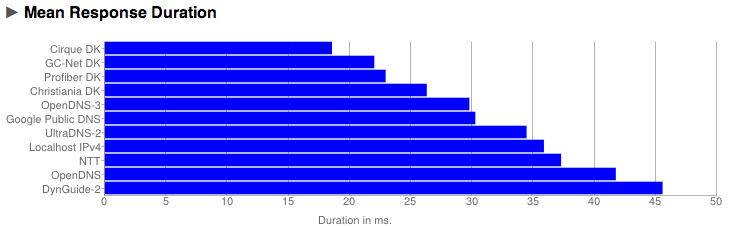
\includegraphics[scale=0.5]{Figurer/NamebenchTest.png}
\caption{Output from Google Test Bench test}
\end{figure}

The test shows, that Cirque DK have the lowest mean response time with 18ms, and the systems localhost DNS have a mean response time on 36ms. One of the more popular public DNS is openDNS, which is a little faster than localhost with 29ms. To test if one of the public DNS is faster than localhost, a test have been made with 5 different internet sites and their given response time. 

To test the given servers, the file located at /etc/bind/named have to be edited. There the given DNS servers adress is typed in, and the BIND server will forward to the given DNS, if the adress is not avaliable on the BIND server. (skal måske rykkes ned / vise figur her?)


\begin{center}
  \begin{tabular}{ l | c  | r}
    \multicolumn{3}{c}{No Forwarding}  \\
	\hline Site & First test (ms) & Second test (ms) \\     
    \hline
    Ubuntu.com & 600 & 826  \\ \hline
    Bt.dk & 218 & 352  \\ \hline
	Iha.dk & 288 & 179 \\ \hline
	Facebook.com & 348 &	240 \\ \hline
	Wikipedia.org & 30 &	50 \\ \hline
  \end{tabular}
\end{center}

\begin{center}
  \begin{tabular}{ l | c  | r}
    \multicolumn{3}{c}{Forwarding - Cirquie.DK}  \\
	\hline Site & First test (ms) & Second test (ms) \\     
    \hline
    Ubuntu.com & 391 & 381  \\ \hline
    Bt.dk & 356 & 906  \\ \hline
	Iha.dk & 375 & 240 \\ \hline
	Facebook.com & 354 &	207 \\ \hline
	Wikipedia.org & 375 & 442 \\ \hline
  \end{tabular}
\end{center}

\begin{center}
  \begin{tabular}{ l | c  | r}
    \multicolumn{3}{c}{Forwarding - OpenDNS}  \\
	\hline Site & First test (ms) & Second test (ms) \\     
    \hline
    Ubuntu.com & 355 & 352  \\ \hline
    Bt.dk & 792 & 436  \\ \hline
	Iha.dk & 334 & 117 \\ \hline
	Facebook.com & 184 & 279 \\ \hline
	Wikipedia.org & 153 & 115 \\ \hline
  \end{tabular}
\end{center}

The tabels show, that Cirquie.DK have a faster response time with 4 out of the 5 test sites than openDNS, which mean that the most optimal public DNS server from the test would be Cirquie.DK. 

(skal vi sammenligne med localhost også eller?)
Slut af med figur om hvordan den spørger??

\subsection{Local filtering}
TODO - Skal skrives om hvordan man kan udbygge filtering ved localhost og spærre for decideret sider. 

\section{Setup BIND Server}
To install a BIND server on Linux type in "sudo apt-get install bind[9]". This will install version 9 of the BIND server software. To check if installation if succesfull type "named -v" and if it is successfull, it will show "BIND 9.8.1-P1". For testing purpose, "dnsutils" have been used - and this can be used to see Query time for the DNS lookup with the commannd "dig -x IP-Adress". 

\end{document} 